\documentclass{beamer}
\beamertemplatenavigationsymbolsempty
\usecolortheme{beaver}
\setbeamertemplate{blocks}[rounded=true, shadow=true]
\setbeamertemplate{footline}[page number]
%
\usepackage[utf8]{inputenc}
\usepackage[english]{babel}
\usepackage{amssymb,amsfonts,amsmath,mathtext}
\usepackage{subfig}
\usepackage[all]{xy} % xy package for diagrams
\usepackage{array}
\usepackage{multicol}% many columns in slide
\usepackage{hyperref}% urls
\usepackage{hhline}%tables
% Your figures are here:
\graphicspath{ {fig/} {../fig/} }

%----------------------------------------------------------------------------------------------------------
\title[\hbox to 56mm{Feature generation}]{Identification of the relationship between labels using an algorithm based on self-attention for temporal sets prediction.}
\author[G.\,L.~Boeva]{Galina Boeva}
\institute{Moscow Institute of Physics and Technology}
\date{\footnotesize
\par\smallskip\emph{Course:} My first scientific paper\par (Strijov's practice)/M05-304 %821, 813
\par\smallskip\emph{Expert:} Ph.D. A.~Zaytsev
\par\bigskip\small 2024}

%----------------------------------------------------------------------------------------------------------
\begin{document}
%----------------------------------------------------------------------------------------------------------
\begin{frame}
\thispagestyle{empty}
\maketitle
\end{frame}
%-----------------------------------------------------------------------------------------------------
%\begin{frame}{Goal of research}
%..
%\end{frame}
%-----------------------------------------------------------------------------------------------------
\begin{frame}{One-slide talk}
\textbf{Data}: Timestamped events characterized by sets of labels - $S^t = \{(X_{j}, Y_{j})\}_{j = t - \tau}^{t-1}$
\centering
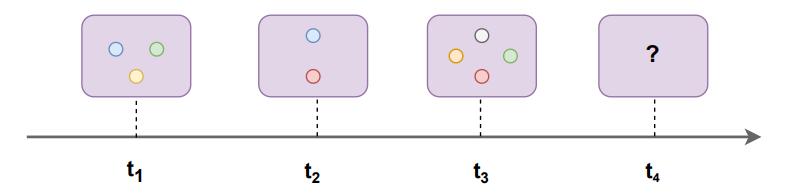
\includegraphics[width=0.7\textwidth]{slide1.png}

\textbf{Goal}: predict labels for the next event
$$
f(X_{t - \tau}, \ldots, X_{t-1}, Y_{t - \tau}, \ldots,  Y_{t-1}, \textbf{z}) \in [0, 1]^K $$
\begin{columns}[c]
\column{0.4\textwidth}

In our case we use cross-entropy loss
\column{0.7\textwidth}
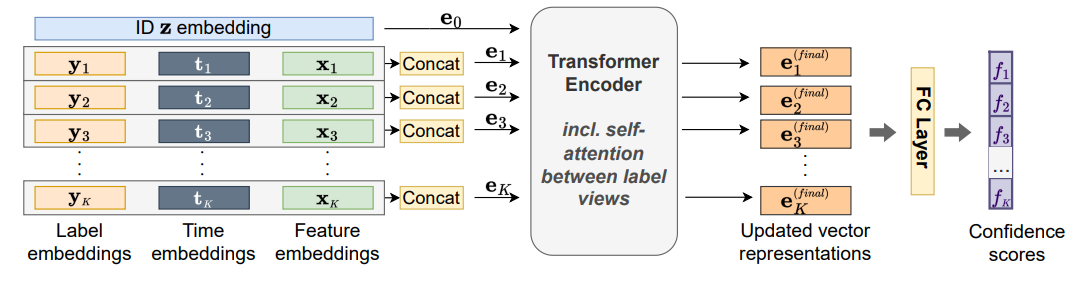
\includegraphics[width=\textwidth]{slide2.png}

\end{columns}
\bigskip

\end{frame}



\end{document} 
